\chapter{Iso-Octane Model}
\section{Kinetic Model}

Liquid transportation fuels are continuously used in different applications and the necessity to understand the reactivity of those fuels has been explored extensively in Chapter 1. Now we turn to the actual oxidation of the second primary reference fuel (PRF) of this work, which is iso-octane. Iso-octane is a member of the branched chain hydrocarbons with the functional group alkane (aliphatics). It is a symbolic name of one of the isomers of octane with the name 2,2,4-trimethyl-pentane using the IUPAC nomenclature alongside the Greek root word ``pent" meaning five but with 2-methyl groups on the second carbon and another methyl group on the fourth carbon atom. Thus, iso-octane is an 8-membered carbon atom with an iso-group branched hydrocarbon. The structure of iso-octane looked at in this work is of 2,2,4-trimethyl-pentane in the skeletal structure of fig.\ref{fig:iso-octane}. Iso-octane has the molecular formula of \ce{C_8H_18} since it is a member of the alkane family with a general structural formula of \ce{C_nH_{2n+2}}. 

\begin{figure}
    \centering
    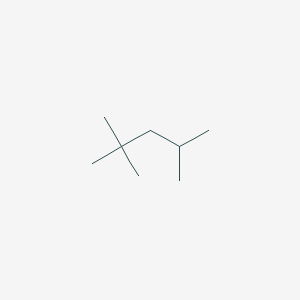
\includegraphics[scale=0.5, keepaspectratio]{images/2,2,4-Trimethylpentane_300.png}
    \caption{Iso-octane Structure}
    \label{fig:iso-octane}
\end{figure}

\vspace{2.5cm}


Iso-octane has long been identified as a constituent compound in the representation of transportation fuels \cite{Dooley2010AProperties}. Since it is representative of the important compounds in transportation fuels, enormous work has been done on the auto-ignition characteristics of the fuel. Experimental investigation of iso-octane includes ignition delay time measurements in shock tubes and rapid compression machines (RCM)  \cite{Fieweger1994Shock-tubePressures}\cite{Fieweger1997Self-ignitionPressure}\cite{Malewicki2013ExperimentalIso-octane}
\cite{Gauthier2004ShockMixtures}\cite{Hartmann2011Auto-ignitionModeling}, laminar flame speeds and flows \cite{BRADLEY1998126}\cite{KUMAR2007209}\cite{Li2012LaminarMixtures}\cite{Hui2013LaminarPressures}\cite{Bieleveld2009ExperimentalFlows}, chemical structure from pyrolysis and oxidation in pressure flow reactors \cite{Gokulakrishnan2007ExperimentalConditions}\cite{Jahangirian2012APressures}, oxidation and pyrolysis in shock tubes \cite{Malewicki2013ExperimentalIso-octane}\cite{Tekawade2016Time-resolvedN-dodecane} and oxidation in a jet stirred reactors \cite{Dagaut2015TheStudy}\cite{Dagaut2014CombustionModeling}\cite{Dagaut2008OxidationStudy}. These experimental measurements provide a basis with which to compare chemical kinetic models of iso-octane as means of validating the mechanisms. Similarly, several kinetic models of iso-octane have been published over the years with Ranzi et al \cite{Ranzi1997AOxidation}, publishing a semi-detailed model similar to n-heptane, Curran et al. \cite{Curran2002AOxidation}, showing the detailed low temperature and high temperature pathways, models have also been published on iso-octane using the CHEMKIN suite code from Malewicki et al \cite{Malewicki2013ExperimentalIso-octane}, iso-octane model has also been deduced based on surrogate modeling of jet aviation fuels using a three-component fuel surrogate model of n-decane, iso-octane toluene as described by Dooley et al \cite{Dooley2010MethylModel}. Westbrook et al \cite{Westbrook2009AN-hexadecane} published a combined model of \ce{C7} to \ce{C16}, Wang et al then constructed a very detailed model that integrates various fuels including n-alkane, cycloalkanes and alkyl-cycloalkanes in the JetSurF v2.0 model \cite{Wang2010A2.0},Sarathy et al followed up with a more compact model of \ce{C_7} to \ce{C_{20}} \cite{Sarathy2011ComprehensiveC20}.Although, skeletal models of iso-octane have been built in the past by Hartmann et al. \cite{Hartmann2011Auto-ignitionModeling}, based on the semi-detailed model of iso-octane and n-heptane Andrae et al. \cite{ANDRAE2008696} built. More recently, Atef et al \cite{Atef2017AKinetics} built a comprehensive iso-octane model with improved thermochemistry parameters and new isomerization pathways. All these iso-octane models built have been validated against various experimental conditions and there is still ongoing work to the determination of new pathways, reaction intermediates, better estimation of thermo-chemical parameters and rate constants for these kinetic models of iso-octane
. \par
\vspace{0.5cm}
The iso-octane model conditions as constructed in RMG have been outlined in Chapter 2 table \ref{tab:PRF_table1} as well as the reactor conditions used in table \ref{tab:PRF_table2} and table \ref{tab:PRF_table3}. This section is going to focus exclusively on the reaction pathways of iso-octane from high-temperature reaction to low-temperature as well as the flux diagram of fig. \ref{fig:f2} of the RMG model validated against published experiments with comparison to other published iso-octane kinetic models. The iso-octane model constructed in RMG was done on the basis of seed mechanisms of 
Burke et al\cite{Burke2012ComprehensiveCombustion}, Hashemi et al\cite{Hashemi2016High-pressureMethane} and Li et al\cite{Li2017TheoreticalC2H4} in the exact order as shown. The major reaction pathways shown in fig.\ref{fig:n-alkane-pathway} were discovered using the schematic and work of Merchant et al.\cite{Merchant2015UnderstandingPropane}, which used propane as a basis for the discovery of reaction pathways. As a result of this discovery, Merchant et al. concluded that the same scheme could be applied to n-alkanes and iso-alkanes up to \ce{C12} with an additional product of cyclic ethers from the \ce{QOOH} radical when they undergo cyclic ether formation reactions - where radicals move from one hydrogen to the other and a ring is formed as well as the loss of the \ce{OH} radical.



\newpage

\section{Reaction Pathways of Iso-octane Kinetic Model}
Iso-octane follows the class of reactions for its oxidation starting with a unimolecular fuel decomposition then a hydrogen abstraction reaction, and further down through a series of steps. H-abstraction reactions occur at both high and low temperatures. These class of reaction was proposed by Curran et al.\cite{Curran2002AOxidation} in the oxidation mechanism of iso-octane. At high temperatures, H-abstraction reactions occur via a $\beta$-scission - simply meaning that when the H-atom is removed, the radical is formed on the adjacent carbon atom to ensure thermodynamic stability and provide less steric hinderance to subsequent reacting species. Nonetheless, since at high temperatures, there is sufficient energy and collisions occur more rapidly, the radical though stable isomerizes and forms other radicals within the other akly groups of the radical atom with molecular formula \ce{C8H17}. The radical site varies depending on where the H-atom was removed. The easiest leaving sites are where the radical is stabilized by more substituted groups. Thus, radical sites that have a primary ($1^{\circ}$) H-atom are less favorable than those of the a secondary ($2^{\circ}$) H-atom and eventually a tertiary ($3^{\circ}$) H-atom. The radical sites with the most favorable H-atom abstractions are shown in fig.\ref{fig:ic8-radicalsites} leading to four distinct radicals of iso-octyl.
\begin{figure}[!htp]
    \centering
    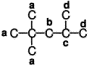
\includegraphics[keepaspectratio]{images/ic8-radical-sites.png}
    \caption{Radical sites for possible H-atom abstraction in iso-octane. Figure from \cite{Curran2002AOxidation}}
    \label{fig:ic8-radicalsites}
\end{figure}

These radicals eventually decompose further along the \ce{C-C} bonds and letting go of yet another hydrogen to form a double bond - olefins with another radical species, thus having a combination of
  \reaction{C-C-C^. \rightleftharpoons C=C + C}
This reaction family in RMG is represented as the R\textunderscore Addition\textunderscore MultipleBond.  Conversely, at low temperatures, the five decyl radicals first decompose again along the \ce{C-C} bond to form smaller alkyl radicals via the R\textunderscore Recombination reaction and these smaller alkyl radicals undergo reaction with \ce{O2} to form alkyl-peroxide radicals or \ce{ROO^.}. The various stages of the reactions are dependent on temperature, thus at higher temperatures the chain branching is not as complex, however at lower temperature many reaction pathways are possible. Since RMG has its own unique class of reaction families that assist in determining which reaction classes guide the fuel molecule to the products desired, we adopt Merchant et al.'s \cite{Merchant2015UnderstandingPropane} guide to following the oxidation of n-alkane and iso-octane fuels using the schematic of fig.\ref{fig:n-alkane-pathway} gives a pictorial illustration to find out the major reaction pathways of iso-octane, especially at low temperatures. In addition, since the onset of ignition in the Negative Temperature Coefficient (NTC) region is of interest, we use the illustration of Merchant et al.\cite{Merchant2015UnderstandingPropane} and Curran et al.\cite{Curran2002AOxidationc} to discover the pathways of low temperature reaction classes of iso-octane. The summary of the reaction classes as proposed by Curran et al.\cite{Curran2002AOxidation} and the corresponding RMG reaction families that enable the discovery of those pathways.





The major reaction classes for all the elementary reactions include the following:
\begin{enumerate}
    \item Unimolecular fuel decomposition
    \item H-atom abstraction from the fuel
    \item Alkyl radical decomposition
    \item Alkyl radical + \ce{O2} to produce olefin + \ce{HO2} radical directly
    \item Alkyl radical isomerization
    \item Abstraction reactions from olefin by OH, H, O and \ce{CH3}
    \item Addition of radical species to olefin 
    \item Alkenyl radical decomposition
    \item Olefin decomposition 
    \item Addition of alkyl radicals to \ce{O2} 
    \item Alkyl peroxy radical isomerization \ce{RO_2 \rightleftharpoons RO_2H}
    \item R\ce{O2^{.} + HO_2^.=RO_2H + O_2}
    \item R\ce{O_2^{.} + H2O2=RO2H + HO_2^.}
    \item R\ce{O2^{.} + CH3O2^{.}=RO^{.} + CH3O^{.} +O2}
    \item \ce{RO2^{.} + $R^\prime$O2^{.} = RO^{.} + $R^\prime$O^{.} + O2}
    \item \ce{RO2H=RO^{.} + O^{.}H}
    \item \ce{RO^.} decomposition
    \item \ce{Q^{.}OOH=QO+O^{.}H} cyclic ether formation via cyclization of diradical
    \item \ce{Q^{.}OOH}=olefin+\ce{HO2^{.}} (radical site $\beta$ to OOH group)
    \item \ce{Q^{.}OOH}=olefin + carbonyl + \ce{O^{.}H} (radical site $\gamma$ to OOH group)
    \item Addition of O2 to \ce{Q^{.}OOH}
    \item Isomerization of \ce{O2^{.}QOOH} and formation of ketohdroperoxide and \ce{O^{.}H}
    \item Decomposition of ketohydroperoxide to form oxygenated radical species and \ce{O^{.}H}
    \item Cyclic ether reactions with \ce{O^.H} and \ce{HO2^.}
\end{enumerate}
 
\begin{figure}
\hspace*{-3cm}
    \centering
    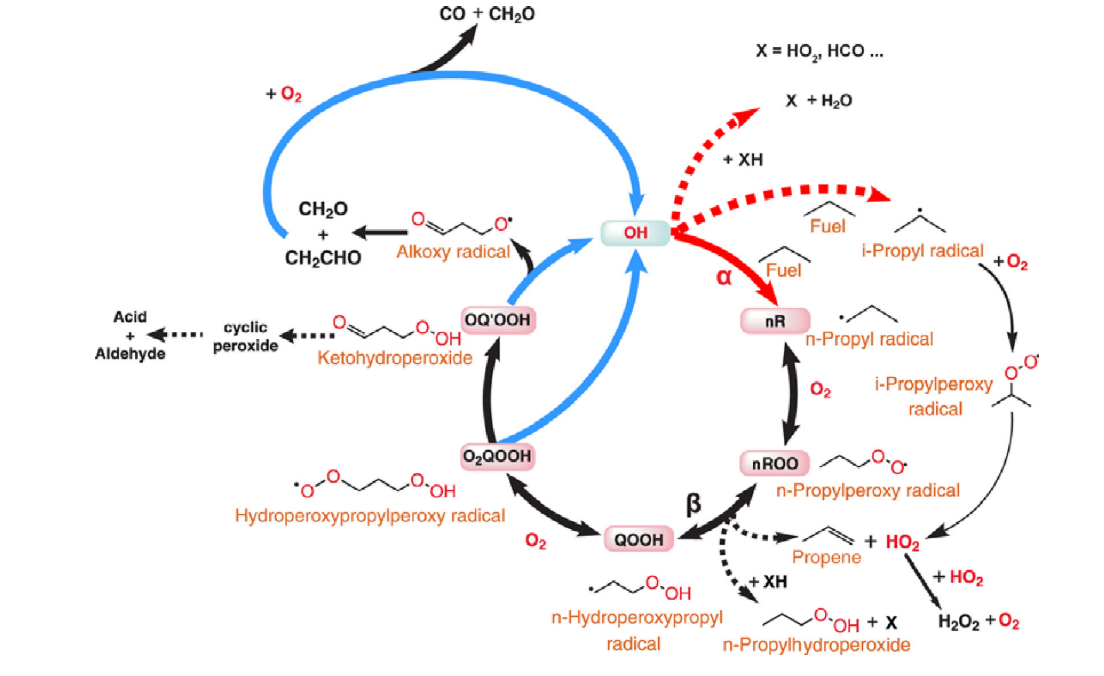
\includegraphics[scale=0.4, keepaspectratio]{images/rxn_class.png}
    \caption{Schematic of Merchant et al.\cite{Merchant2015UnderstandingPropane} major reaction pathways of propane during the first-stage of ignition. Reactions in blue lead to the formation of OH radicals. The reactions in dotted lines show competing pathways that divert radicals and lead to delay in the first-stage ignition}
    \label{fig:n-alkane-pathway}
\end{figure}

The convention of naming in this work is the R refers the the complete iso-octane mechanism while $R^\prime$ refers to the alkyl radical as seen in \ce{C^.}, Q refers to the isomerized form of \ce{ROO^.} via an intra H-migration reaction with molecular formula \ce{C_nH_{2n}}. For the reaction classes, the rates used are those from the reaction libraries as outlined in the summary of table \ref{tab:PRF_table1} and the seed mechanisms also outlined in table \ref{tab:PRF_table1}.

\cleardoublepage

\subsection{High Temperature Mechanism}

The high temperature mechanism can be accurately described with reaction classes 1-9.
\subsubsection{Unimolecular Fuel Decomposition and H-Abstraction Reactions} 
These reactions produce five alkyl radicals with the radical changing from one carbon atom to the next as well as an extra \ce{H} atom. Since the H atom abstraction reactions require high activation energies, they tend to favor the reverse direction as they serve as sink of H atoms. This initiation reactions are often observed in high temperature and pressure experiments such as that of shock tubes. In RMG, this reaction family is described by the H-Abstraction family with the general form 

\reaction{R^{1}-H^{2} + R^{3}\cdot \rightleftharpoons R^{1}\cdot {+} H^{2}-R^{3}\hspace{1cm} \text{H\textunderscore Abstraction reaction family}}

The four distinct iso-octyl radicals are show in fig.\ref{fig:iso-octyl_radicals}

\begin{figure}[!htp]
    \centering
    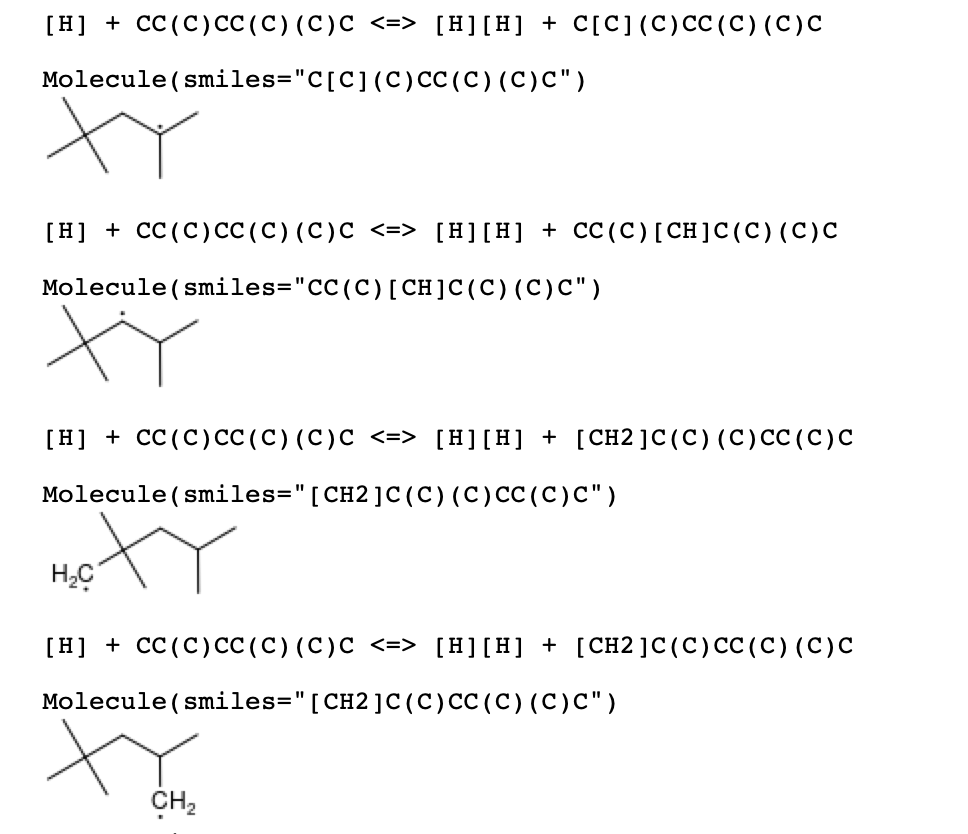
\includegraphics[keepaspectratio]{images/iso-octyl-radicals.png}
    \caption{Iso-octyl radicals from the H-atom abstraction}
    \label{fig:iso-octyl_radicals}
\end{figure}

\subsubsection{Alkyl Radical Decomposition Reactions}
Alkyl radical decomposition reactions involve the breaking of the previously generated alkyl radical along the C-C bonds and is only relevant at high temperatures $>$ 850 K \cite{Curran1998AOxidation}. There is competition usually between this reation pathway and the addition of \ce{O2} to the alkyl radicals because of the low energy barrier for the addition of \ce{O2}, the pathway to give ROO can sometimes be favored. However, for larger alkanes > C8 the breaknig of the alkyl radical usually occurs via the $\beta$-scission to aid for the addition of the \ce{O2}. This reaction often leads to the formation of olefins (alkenes) or C=C double bonds as well as another radical. This reaction family is described in the RMG reaction family as radical recombination as the breaking down of the C-C bond usually favors the reverse direction with a general form as this 

\reaction{{R^{1}\cdot {+} R^{2}\cdot \rightleftharpoons R^{1}-R^{2}} \hspace{1cm} \text{R\textunderscore Recombination reaction family}}

\subsubsection{Alkyl Radical + \ce{O2} = Olefin + \ce{HO2^{.}} and Alkyl Radical Isomerization Reactions}

The reaction of alkyl radicals with \ce{O2} can undergo through various reaction paths. The reaction channel usually involves the addition of \ce{O2} in the form of \ce{O^{.}-O^.} where Oxygen is represented as a biradical singlet since this is the most stable form in its electronic structure. This reaction adds to the alkyl radical via the radical recombination channel and forms a alkylperoxy radical which then undergoes an isomerization to form a hydroperoxy-alkyl radical with the loss of a hydrogen atom. This new form is often labeled as \ce{QOOH} where the Q usually denotes the presence of a double bond. The reaction family of the first step from alkylperoxy radical to hydroperoxy-alkyl radical is the intra\textunderscore H\textunderscore migration and then finally to form the double bonded olefin is the R\textunderscore Addition\textunderscore MultipleBond.

\reaction{{H^{3}-R^{2}\thicksim R^{1}\cdot \rightleftharpoons R^{2}\cdot\thicksim R^{1}-H^{3}} \hspace{1cm} \text{intra\textunderscore H\textunderscore migration reaction family}} 
\reaction{R^{2}=R^{1} + R^{3}. \rightleftharpoons R^{2}.-R^{1}-R^{3}\hspace{1cm} \text{R\textunderscore Addition\textunderscore MultipleBond reaction family}}

The \ce{ROO^.} radicals are shown in fig.\ref{fig:iso-octyl-peroxy radicals} when \ce{O2} is added to the iso-octyl radicals and during the inner H-atom migration process isomerizes to the iso-octyl-hydroperoxy radicals \ce{Q^{.}OOH} shown in fig.\ref{fig:ic8-QOOH}.

\begin{figure}[!htp]
    \centering
    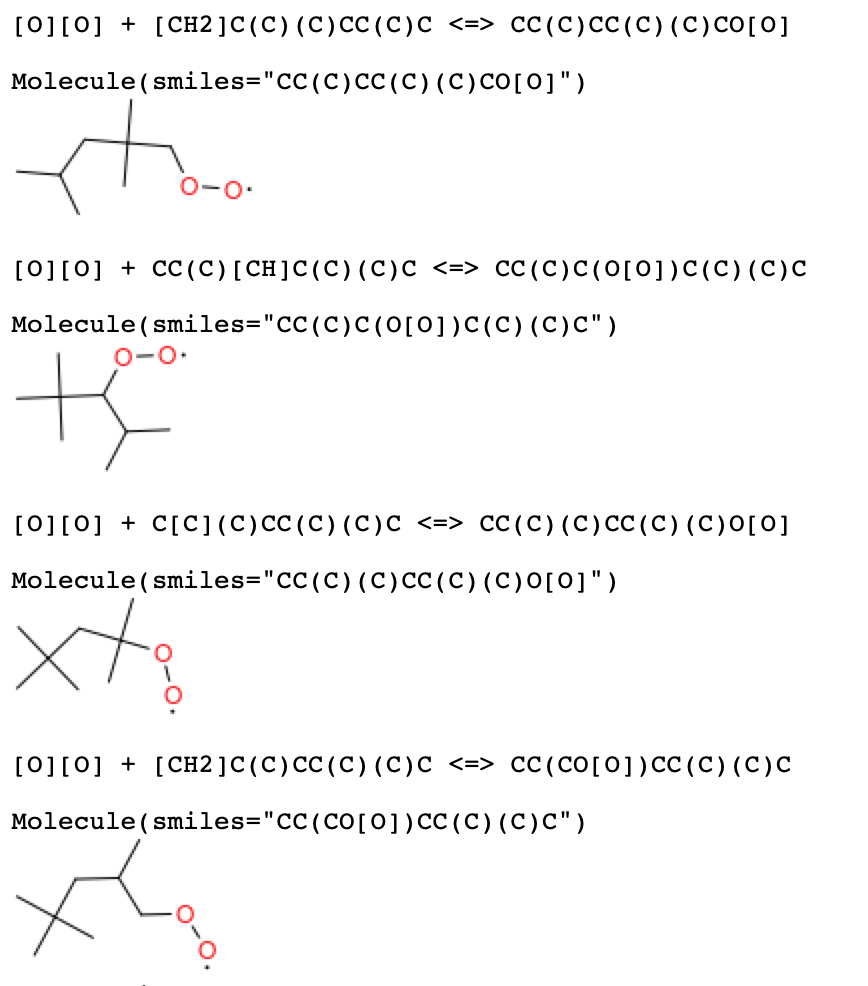
\includegraphics[scale=0.45, keepaspectratio]{images/iso-octyl-ROO.png}
    \caption{Iso-octylperoxy radicals }
    \label{fig:iso-octyl-peroxy radicals}
\end{figure}

\begin{figure}[!hbp]
    \centering
    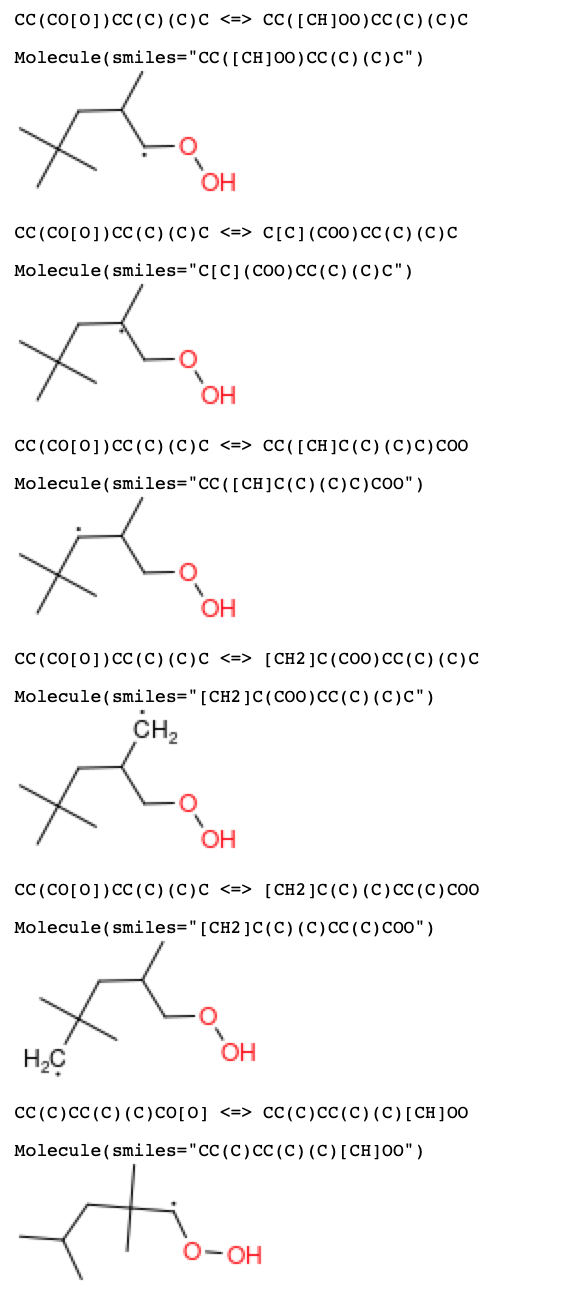
\includegraphics[scale=0.45, keepaspectratio]{images/iso-octyl-QOOH.png}
    \caption{Iso-octyl-hyrdoperoxy radicals \ce{Q^{.}OOH}}
    \label{fig:ic8-QOOH}
\end{figure}

Reaction classes 4-9 deal entirely with reactions of olefins. Since at high temperatures, the steric considerations are complex in the reaction channels, more emphasis is left on this reactions as the rate expressions are very complex in describing the pathways.
\newpage
\subsection{Low Temperature Mechanism}
The low temperature mechanism can be described as reactions at temperatures $<$ 900 K with reaction classes 10-24.

\subsubsection{Addition of alkyl radicals to \ce{O2} and Alkyl peroxy radical isomerization \ce{RO2 \rightleftharpoons RO2H}}

The $\beta$-scission high activation energies makes reactions much slower, thus reactions with lower activation energies take precedence. The first is the addition of oxygen \ce{O2} to the alkyl radical and then isomerization reactions on the ROO radicals occur throughout the radical moving the radical sites with a \ce{H}-atom shift (internal H-abstraction) on the radical. 
\reaction{H^{3}-R^{2}\thicksim R^{1}\cdot \rightleftharpoons R^{2}\cdot\thicksim R^{1}-H^{3} \hspace{1cm} \text{intra\textunderscore H\textunderscore migration reaction family}} However, these internal H-abstraction reactions (H-migrations) are rather slow at lower temperatures thus making the addition of ROO decomposition to yield two reactive reactive hydroxyl radical and a carbonyl group. Evidently, Pollard \cite{Pollard1977Hydrocarbons} carried out extensive low temperature kinetic analysis of hydrocarbon oxidations and mapped out the most important features of low temperature submechanism. Many recent models have integrated these features in their models for simplifications essential for the oxidation of low temperature hydrocarbons. 



\subsubsection{Radical decomposition of \ce{RO2H \rightleftharpoons RO^{.} + O^{.}H} and \ce{Q^{.}OOH \rightleftharpoons QO + O^{.}H} }
The first step of the decomposition of \ce{RO2H} alkyl-hydroperoxides is one of the very important steps in the process of hydrocarbons and often controls the onset of a Negative temperature coefficent (NTC) regime in the auto-ignition of hydrocarbons. Thus, the production of the \ce{O^{.}H} radicals is necessary for the first-stage ignition process \cite{Merchant2015UnderstandingPropane} as well as the optimization process for cetane sensitizer improvements \cite{Curran1998AOxidation}. In order to form the alkenyl-hydroperoxy radicals \ce{Q^{.}OOH} from the alkyl-peroxides \ce{RO2}, unimolecular isomerizations occur again via the intra\textunderscore H\textunderscore migration reactions. 

When the alkoxy radicals are produced \ce{RO^.} from the decomposition of the alkyl-hydroperoxides \ce{RO2H}, they often tend to be unstable and decompose more readily to the stable form of oxygenated alkoxy radicals for large carbon chains often $>$ C8 with the presence of carbonyl groups such as aldehydes and ketones and other smaller alkoxy radical species via the intra\textunderscore H\textunderscore migration reaction family. The smaller alkyl radicals decompose even further eventually following a $\beta$-scission to form olefins (alkenes) via the R\textunderscore Addition\textunderscore MultipleBond reaction family, which is stable in this form by the presence of its pi bonds. For the aldehydes, due to the presence of a double bonded oxygen, they are reactive and additions to the double bond are possible forming yet another alkyl radical and another oxygen radical which can attack double bonds. 


As the radical decomposition continues, the alkenyl-hyrdoperoxy radicals involves the breaking of the \ce{O-O} bond with the chain branching to form cyclic ethers with an extra \ce{O} atom in the chain.As the chain branching begins, cyclic ethers are formed with the loss of the internal \ce{H} from QOOH as a competing reaction pathway. The cyclic ether formation has a unique reaction family in the RMG database that forms from the \ce{QOOH} radical seen as \reaction{R^{1}^.\thicksim O^{2}-O^{3}-R  \rightleftharpoons R^{1}\thicksim O^{2} + O^{3}R^. \hspace{1cm} \text{Cyclic\textunderscore Ether\textunderscore Formation }} The presence of these cyclic ethers is shown in the schematic of Merchant et al.\cite{Merchant2015UnderstandingPropane} fig.\ref{fig:cyclic-ethers}. 

\begin{figure}[!ht]
\hspace*{-3cm}
    \centering
    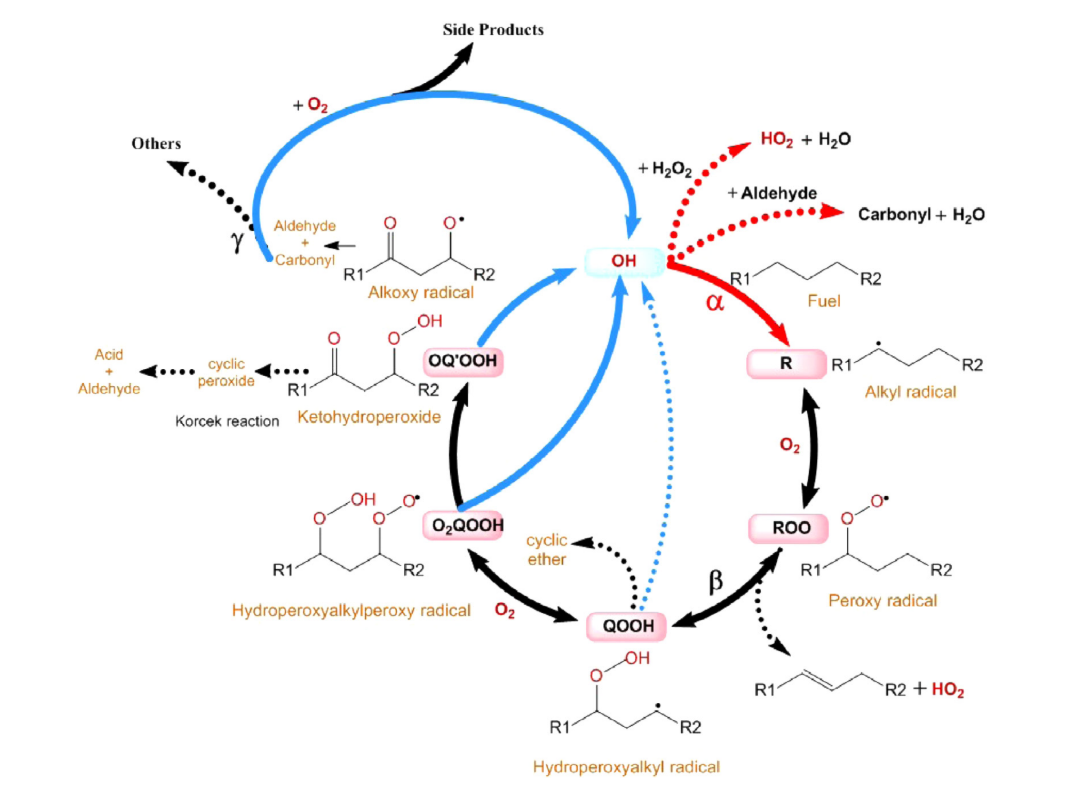
\includegraphics[scale=0.45, keepaspectratio]{images/nalkane-schematic+ROR.png}
    \caption{Schematic of low temperature oxidation of n-alkanes with the presence of cyclic ethers as shown by Curran et al.\cite{Curran1998AOxidation} and schematic from Merchant et al.\cite{Merchant2015UnderstandingPropane}}
    \label{fig:cyclic-ethers}
\end{figure}


\subsubsection{Decomposition of \ce{Q^{.}OOH \rightleftharpoons Olefin + HO2^.} and \ce{Q^{.}OOH \rightleftharpoons Olefin + Carbonyl + O^{.}H}}

Alkenyl-hydroperoxide radicals \ce{Q^{.}OOH} have a $\beta$ radical site that can decompose to an olefin and hydroperoxy radical \ce{HO2^{.}} via an addition reaction along the \ce{Q-OOH} site. The \ce{HO2^.} radicals often play an important role in the auto-ignition process of hydrocarbons and contributes to the NTC behavior of n-decane. Similarly, rather than decomposition along the \ce{Q-OOH} site, $\beta$-scission can occur and the presence of olefins alongside a smaller carbonyl group usually a ketone and a hydroxy radical \ce{O^.H} is formed. These three body reactions usually have very high weak dependence on temperature and its rate estimates are often observed to be very close to the high pressure limit and violate the collision limits of the Lennard-Jones parameter as described by Chen et al.\cite{Chen2017ViolationModels}. 


\subsubsection{Addition of \ce{O2} to \ce{Q^.OOH} and Isomerization of \ce{O2^.QOOH} to Ketohydroperoxide and \ce{O^.H} radicals}
Alkenyl-hydroperoxide \ce{Q^.OOH} radicals can react with \ce{O2} via radical recombination reactions to form peroxy alkenyl-hydroperoxide radicals \ce{O2^.QOOH}. \reaction{R^{1}\cdot {+} R^{2}\cdot \rightleftharpoons R^{1}-R^{2} \hspace{1cm} \text{R\textunderscore Recombination reaction family}}
 
 Further chain branching steps of the peroxy-alkenyl-hydroperoxide radicals can form \ce{HOOQ^.OOH} dihydroperoxy-alkenyl radicals via an inernal H migration reaction before the final isomerization reaction to eliminate the \ce{O^.H} radicals and form different ketohyperoxide species depending on the carbon chain. The QOOH radicals alongside chain branching form a combination of carbonyl groups of ketones and olefins as well as OH radicals. The \ce{O2QOOH} species then isomerize to form ketohydroperoxides and OH radicals along the double bonds.  
 
 The full pathways integrating both the high and low temperature chemistry is seen in fig.\ref{fig:f2} of n-decane.

\begin{figure}[!htp]
    \centering
\hspace*{-3cm}
    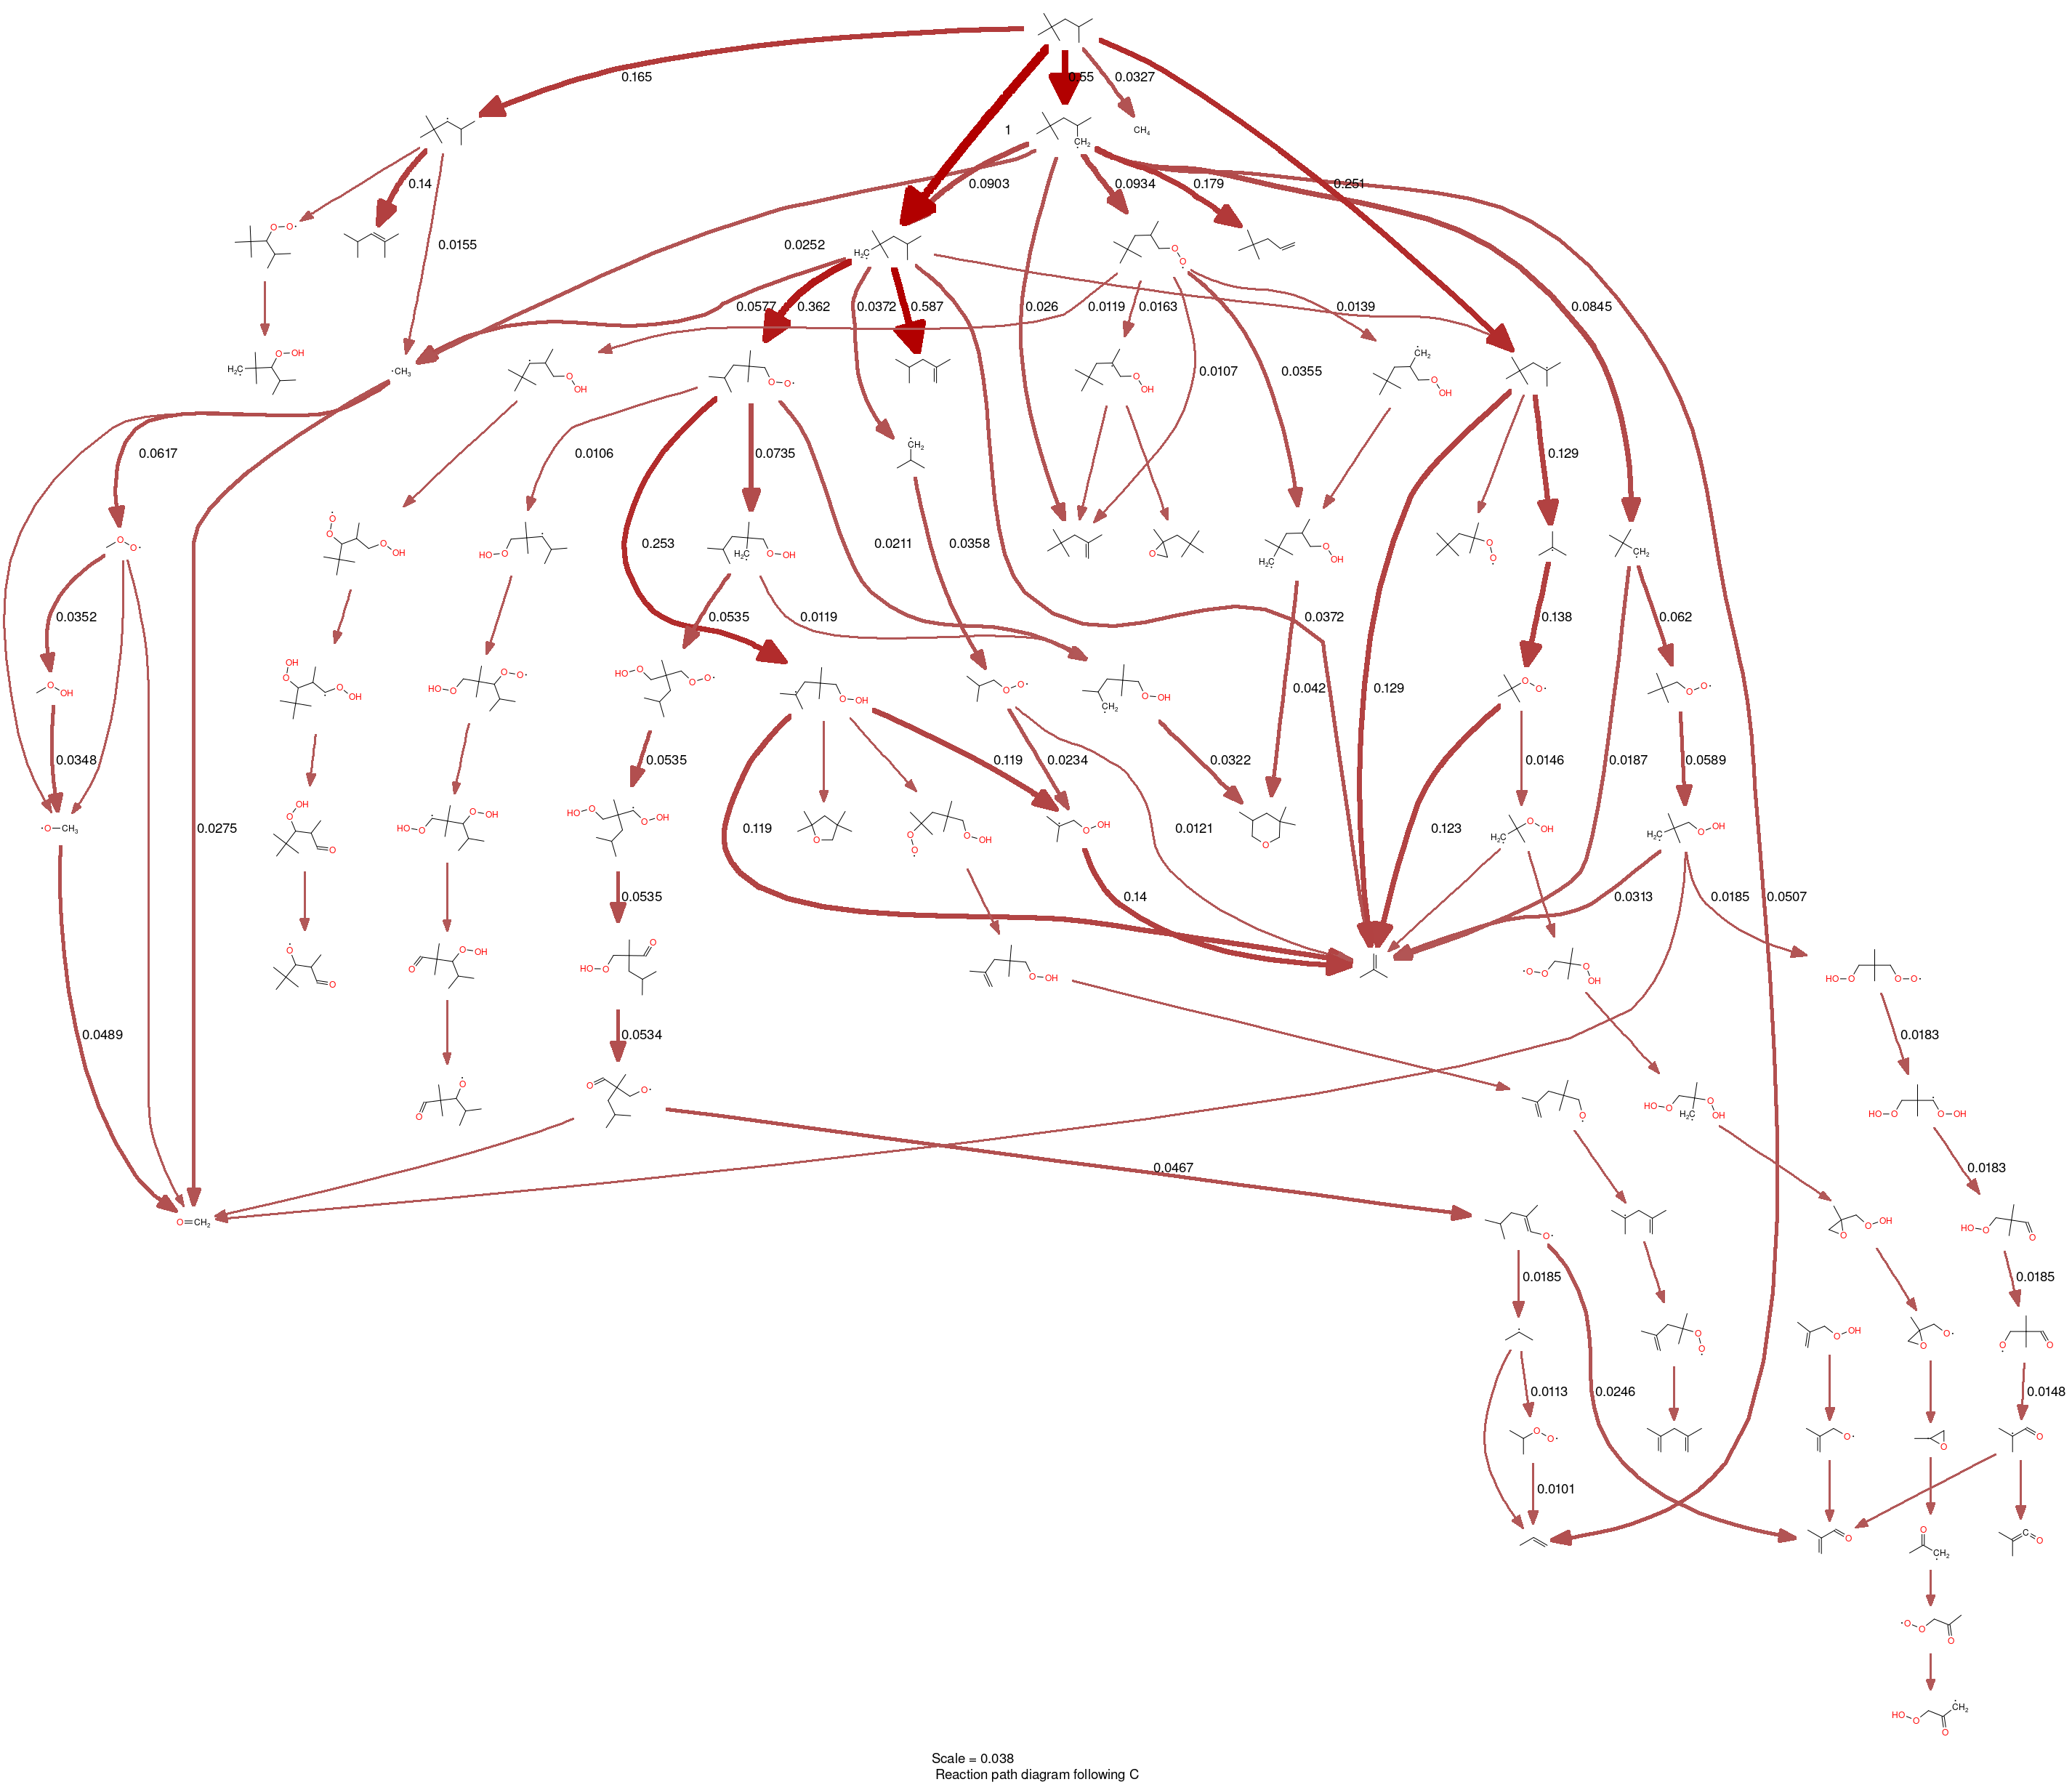
\includegraphics[scale=0.2,keepaspectratio]{images/ic8-flux_pathways.png}
    \caption{Flux diagram of iso-octane @ 800K and 13 bar}
    \label{fig:f2}
\end{figure}

\cleardoublepage

\section{Model validation of iso-octane under experimental conditions}
The detail of the model generation of iso-octane using RMG has been described in sufficient detail with the inclusion of both the high temperature and low temperature reaction pathways as well as the model generation process algorithm highlighted in Chapter 2. Now we look into the validation of the iso-octane model using the chemical kinetics code Cantera \cite{cantera}. The model is only validated against experiments of Shock Tubes for ignition delay time measurements at a wide range of conditions.


\subsection{Model validation of iso-octane in shock tubes for ignition delay time predictions}
Shock tubes essentially devices designed to experiment and study the flow of high-temperature and high-velocity effects of compressible gases within an actual engine-like environment. It is designed on the basis of knowledge of gas dynamics and analysing shock waves. It operates on the principle that at high temperatures, supersonic gases flow is in the tube a diaphragm causes a separation into regions of high-pressure and low-pressure. As the pressure rises, an unsteady rarefied wave passes into the driver gas with a velocity usually a few kilometers per second causing flow from the high-pressure region to the low-pressure region. As the shock wave progresses in the low-pressure region, it pushes the low-pressure gas ahead of it. Thus, creating two fronts, flow ahead of the shock wave and flow behind the shock wave. The flow ahead of the behind the shock wave (driver gas) is the gas of interest. The velocity of the driver gas is equal to  that of the driven gas\cite{Greene1964TheR.}. Usually, there in the high-pressure region, is an explosive gas which is the gas studied, and present is a laser beam to detect the luminescence of some excited species. The ignition delay time can be defined as the time it takes:
\begin{enumerate}
    \item For the shock wave to hit the wall and propagate with the excitation of a \ce{CH*} or \ce{OH*}radical
    \item For the shock wave to hit the wall and measurement of the highest peak of the temperature in the driven section
    \item For the shock wave to hit the wall and detection of the highest peak of the pressure in the driven section
\end{enumerate}
Since all three possibilities of measuring the ignition delay time data in shock tubes exist, it is often well defined based on one of the three main possibilities usually for the first-stage ignition \cite{Davidson2004InterpretingData}\cite{Fieweger1994Shock-tubePressures}\cite{Fieweger1997Self-ignitionPressure}\cite{Pfahl1996Self-ignitionConditions}\cite{Haylett2012IgnitionTube}

In Cantera, this process is often defined based on the reactor type of interest. First, the gas solution object is created with the \textbf{gas.Solution} class, then a reactor type is selected with the appropriate initial conditions usually coming from the experimental data being validated against. Next, the state of the system is set with the reactor network previously defined and then a simulation in time for the next states is found using the ODE solver. The ODE solver starts at the current state  of the systems and progresses in time by one of the following methods:
\begin{enumerate}
    \item \textbf{step()}: This involves a reactor step from the current state of the system by solving the previous state of the system using the time step given. This is an explicit method where the ODE solver internally solves the numerical Differential Algebraic Equations (DAE) system. The new time is returned as well as the state of the system at the next state using the previously defined time step $\Delta$t within the solver absolute and relative tolerances. The time step cannot be larger than the maximum time step or else the ODE solver breaks.
    \item \textbf{advance($t_{new}$)}: This method solves the state of the system at a predefined step times $t_{new}$. This $t_{new}$ describes the absolute time of the system from the initial system by calling the ignition delay time function for the reactor in a loop, either a while loop or for loop at exactly the time specified - basically using the \textbf{step():} function several times in the process. In addition, the \textbf{advance():} function can be made to continue until a steady-state solution is attained by time stepping. Only when the feature-scaled residual of the state vector is below a given threshold value is the system at steady-state and the ODE solver stops.
\end{enumerate} 
For all shock tube models in this work, a zero-dimensional homogeneous closed ideal gas reactor with constant volume and internal energy class was used since at constant volume, there is no P-V work done against the control volume of the gas. Since the temperature is known, the energy equation is computed assuming adiabatic conditions in the reactor volume. The time integration of the species is computed in uniform time steps until the solution is found. During the time integration, the reactor model scheme usually an ODE SUNDIALS solver \cite{hindmarsh2005sundials} solves the differential equations of the species within the energy equation. The energy equation accounts for the energy interaction via the heat equation but is ignored since the reactor assumes adiabatic conditions and indicates only mechanical work interactions, mass transport due to species diffusion and conversion.  The equation being solved in the ideal gas reactor  of Cantera is equation \ref{eq.mass conservation} as given by Robert Kee et al's book on Chemically Reacting Flow \cite{Kee2003ChemicallyPractice}. The definition of the ignition delay time varies. Nonetheless, the model used in Cantera assumes an ignition delay time based on the excited \ce{CH} or \ce{OH} radical species and is often very close to the highest temperature spike Ji et al point out for the sensitivity analysis of ignition delay times \cite{Ji2019EvolutionAutoignition}. 

\begin{equation}
    U = m\sum_k{Y_k u_k(T)}
\end{equation}

\begin{equation}
    \frac{dU}{dt} = u\frac{dm}{dt}+mc_v\frac{dT}{dt}+m\sum_k{u_k \frac{dY_k}{dt}}
\end{equation}

\[\text{Substituting the corresponding derivations for temperature in the reactor as:} \]


\begin{equation}
    mc_v\frac{dT}{dt}=-p\frac{dV}{dt} - Q^. + \sum_{in}{m_{in}(h_{in}- \sum_k{u_k Y_{k, in}}) -\frac{pV}{m}\sum_{out}{m_{out}^.} - \sum_k{m_{k, gen}^. u_k}}
    \label{eq.mass conservation}
\end{equation}

The ignition delay times prediction are presented as modeled in Cantera against shock tube experiments of Fieweger et al.\cite{Fieweger1994Shock-tubePressures}\cite{Fieweger1997Self-ignitionPressure} in fig.\ref{fig:idt times}.

As seen in fig. \ref{fig:idt times}, there is good agreement between the model prediction of ignition delay times against the experiments of Fiewger et al. who studied the self-ignition of several spark-ignition (SI) engine fuels between lean, stoichiometric and rich fuel mixtures under engine-like conditions in a high pressure shock tube and observed a transition from deflagration-like behavior to a  detonation-like behavior around 960 K with strong high pressure peaks, cool flame and onset of a NTC regime in a two-step ignition.


\begin{figure}[!hbp]
    \centering
    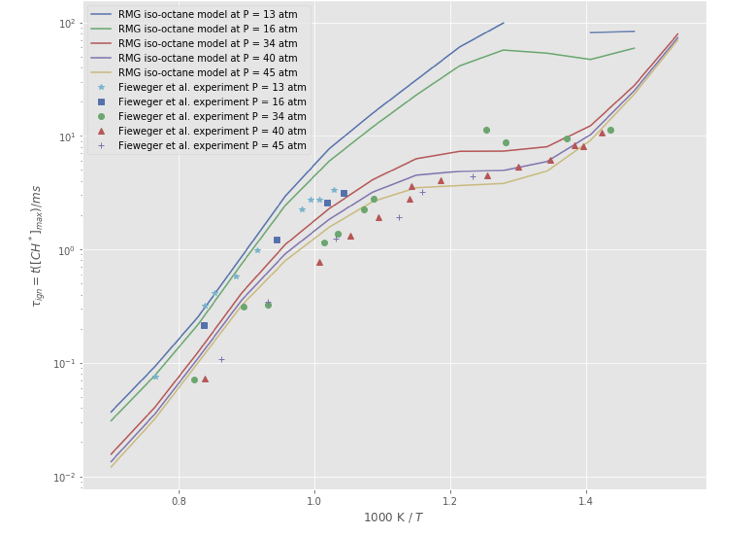
\includegraphics[scale=0.4, keepaspectratio]{images/ic8-idt.png}
    \caption{Ignition delay time prediction of iso-octane/air at 13 atm, 16 atm, 34 atm, 40 atm and 45 atm for $\phi=1$ stoichiometric mixtures against experiments of Fieweger et al. \cite{Fieweger1994Shock-tubePressures}\cite{Fieweger1997Self-ignitionPressure}. Lines indicate model predictions and symbols indicate experiments}
    \label{fig:ic8-idt}
\end{figure}

\cleardoublepage
\subsubsection{Sensitivity Analysis of the Ignition delay times}
A detailed analysis was done to determine which control variables control the ignition delay of the iso-octane model. Since the species usually measured for the onset of ignition is the \ce{OH^.} radical \cite{Ji2019EvolutionAutoignition}, the concentration of the \ce{OH^.} radical was used as the criteria for sensitivity by the use of a brute force method comparing the localised sensitivity at a given temperature for all the top 20 most sensitive reactions that influence the ignition delay time. This sensitivity analysis was done at high temperatures of 1300 K, intermediate temperatures of 900K and at low temperatures of 700K to observe which reactions contribute the most to either the production or consumption of the \ce{OH^.} radical species. 

The sensitivity analysis involves the perturbation of both the forward and reverse rates of the 20 most sensitive reactions to \ce{OH^.} radical concentration by a factor of two and then comparing the change in the ignition delay time to the preset (original )rate constant of those same reaction ignition delay time sensitivity coefficients to the \ce{OH^.} radical species. The magnitude of the sensitivity coefficient indicates a strong dependence on \ce{OH^.} radical concentration, while the sign indicates rate of production if positive and rate of consumption if negative. The sensitivity plots are shown in fig.\ref{fig:ic8-sensitivity}.

The summary of the RMG iso-octane model is given in table \ref{tab:iso-octane_model_summary}. 
\begin{table}[ht]
\arrayrulecolor[HTML]{DB5800}
\caption{Summary of RMG iso-octane model analysis and Ignition delay time prediction at extinction }
\centering
\begin{adjustbox}{width=1\textwidth}
\begin{tabular}{ p{6cm} c c c c }
\rowcolor{lightgray}\multicolumn{4}{|c|}{RMG iso-octane model summary} \\
Number of Species before sensitivity analysis & 492 & &  \\ 
Number of species after sensitivity analysis  & 19558 & &  \\
Number of Reactions before Sensitivity analysis & 19558 & & \\ 
Number of reactions after sensitivity analysis & 19558 & & \\ 
\hline
 Model ignition delay time at extinction &  Temperature & Pressure & Equivalence ratio \\
 \begin{tabular}{ c }
    $\tau$=98.6775 ms   \\
    $\tau$=59.17276 ms \\ 
    $\tau$=78.6791 ms \\
    $\tau$=73.26734 ms \\
    $\tau$=69.76976 ms \\ 
 \end{tabular} & \begin{tabular}{ c } 
       782.1229 K\\
      679.6116 K \\
      651.16279 K \\
     651.16279 K \\
     651.16279 K \\
 \end{tabular} & \begin{tabular}{ c }
      13 bar  \\
      16 bar \\
      34 bar \\
      40 bar \\
      45 bar \\
 \end{tabular} & 1.0 \\
 \end{tabular}
    \end{adjustbox}
    \label{tab:iso-octane_model_summary}
\end{table}


\begin{figure}
    \centering
    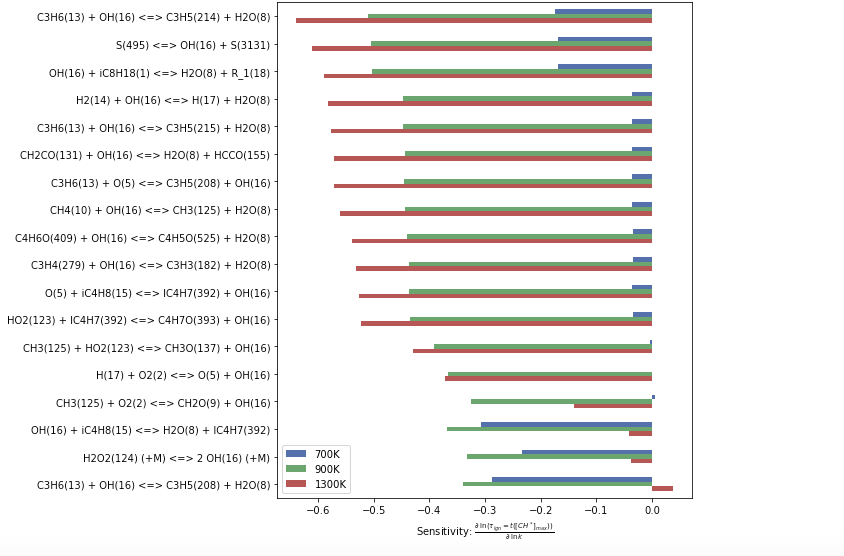
\includegraphics[scale=0.45, keepaspectratio]{images/sensitivity-iso-octane.png}
    \caption{Sensitivity coefficients of the ignition delay time of the iso-decane model to \ce{OH^.} radical concentration at stoichiometric fuel/air mixture at 700 K, 900 K, 1300 K at $P=13$ bar. Where the ignition delay times $\tau_{ign}=t(\ce{CH^.}_{max})$}
    \label{fig:ic8-sensitivity}
\end{figure}


\begin{figure}
    \centering
    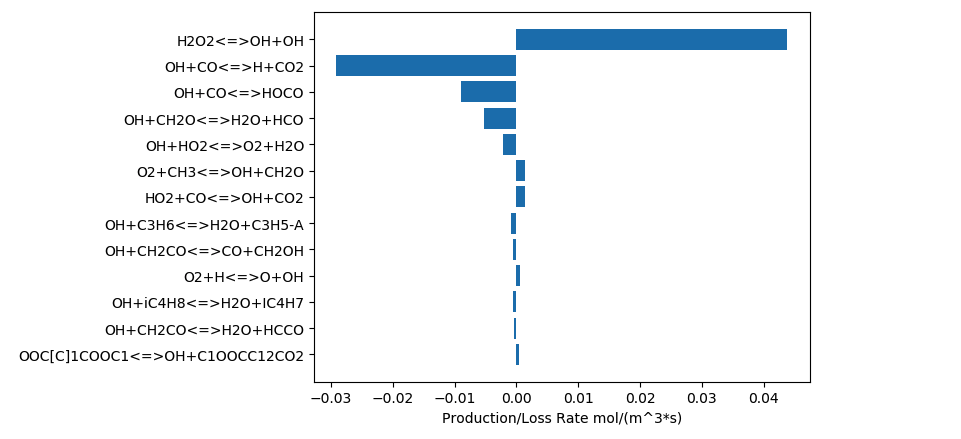
\includegraphics[scale=0.45, keepaspectratio]{images/ic8-ROP.png}
    \caption{Rates of Production/Consumption of the \ce{OH^.} radicals of the iso-octane model}
    \label{fig:rop-nc10}
\end{figure}